In this part, we used a neural network to predict the number of discrete eigenvalues in a nonlinear spectrum of telecommunication signals. The discrete spectrum reflects the internal structure of the signal, and knowledge of this structure allows one to find out the signal properties and the features of its propagation over a nonlinear optical fibre.



\begin{figure}[htpb]
    \begin{minipage}[h]{0.5\linewidth}
    \center{
        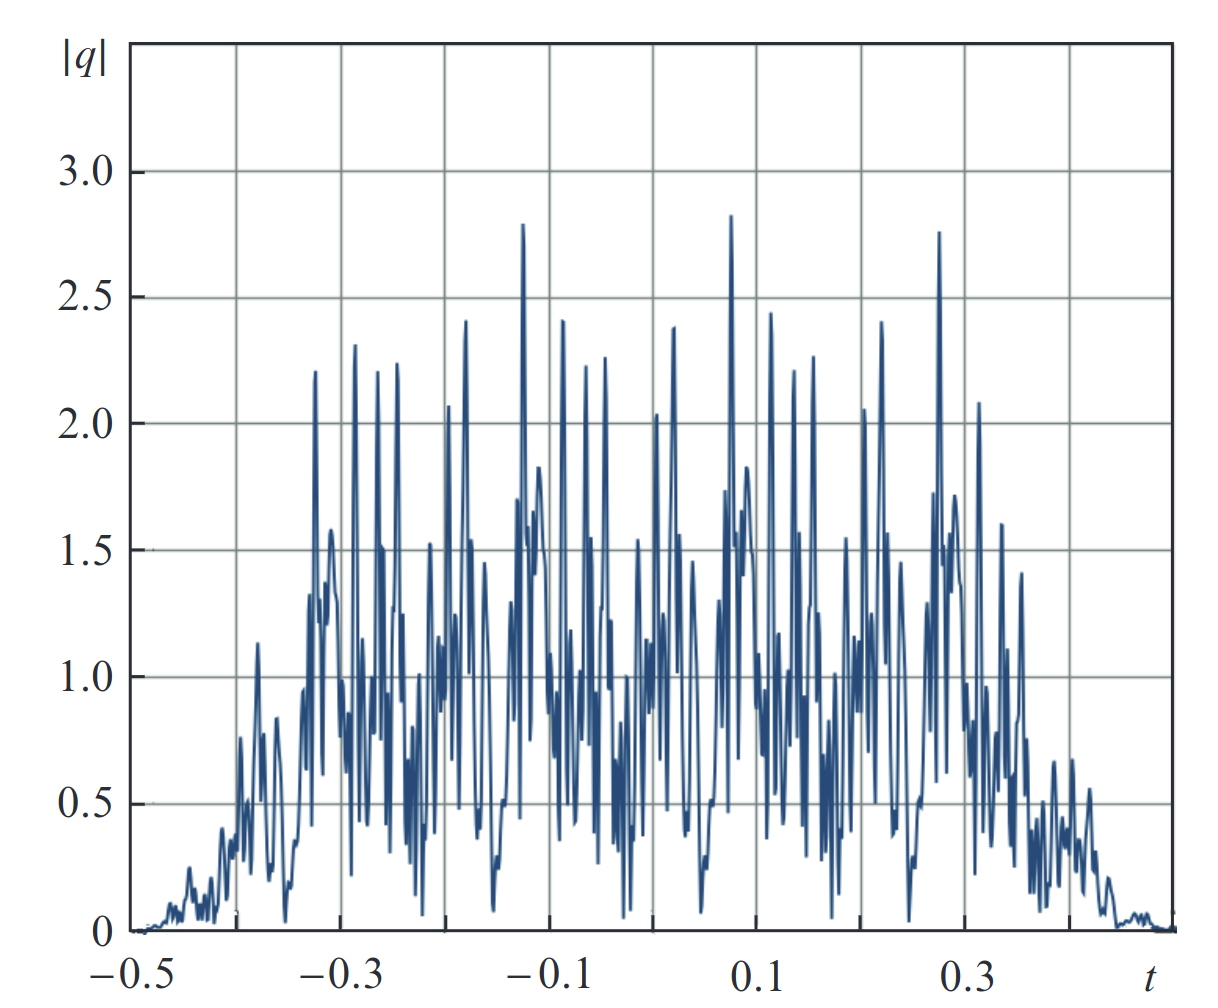
\includegraphics[width=1\linewidth]{images/nn_discrete/signal_example.png} (a) \\
    }
    \end{minipage}
    \hfill
    \begin{minipage}[h]{0.5\linewidth}
    \center{
        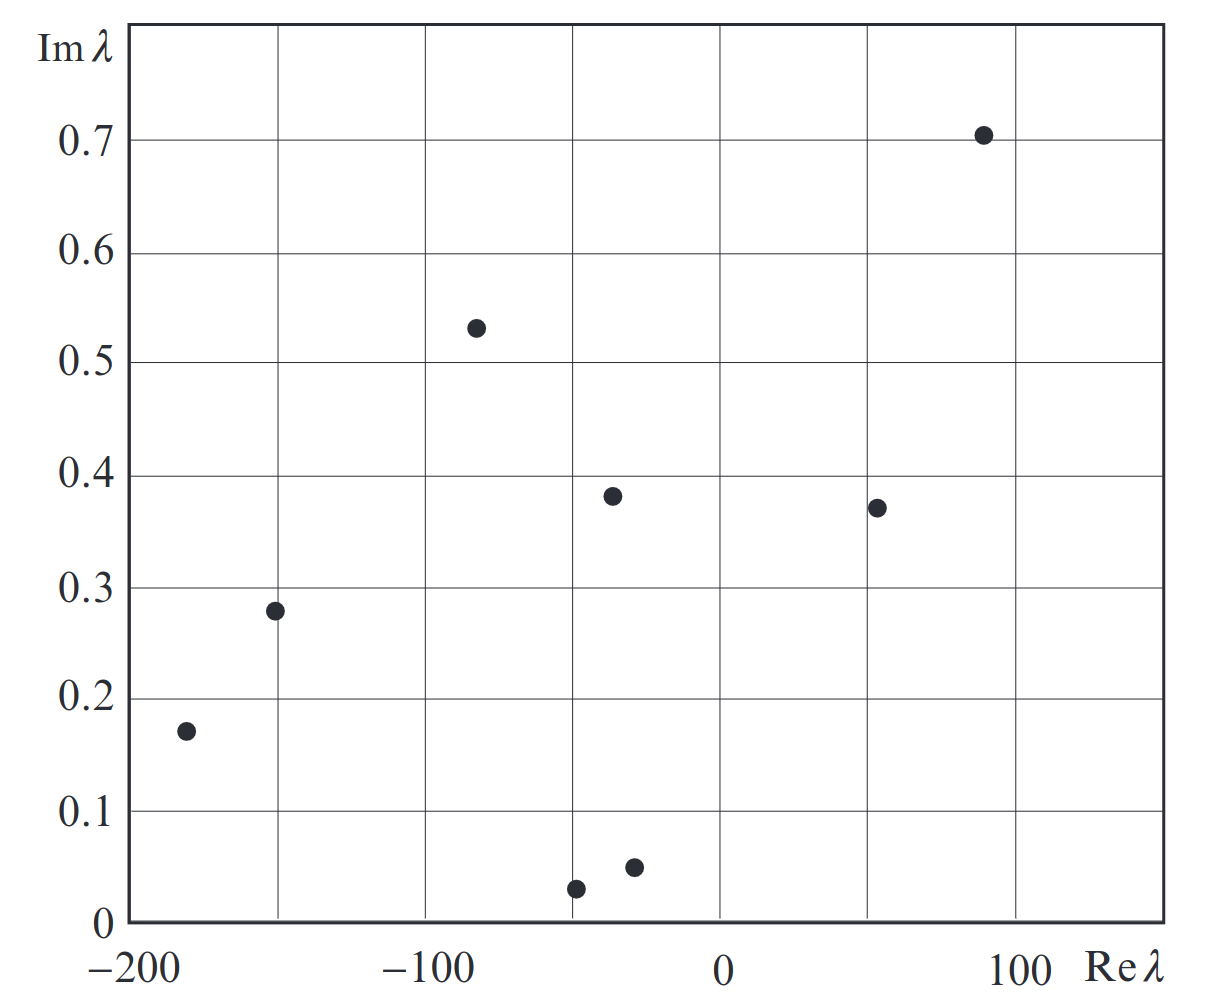
\includegraphics[width=1\linewidth]{images/nn_discrete/spectrum_example.png} (b) \\
    }
    \end{minipage}
    \caption{(a) Example of the dependence of the amplitude of the \acrshort{wdm} signal under study on time (one of the possible implementations is given), and (b) example of the location of the discrete spectrum components in the complex half-plane of the spectral parameter $\xi$ for one of the signals under study.}
    \label{fig:nn_discrete_example}
\end{figure}

The signal was generated from a random dataset encoded in one of the modulation formats for $C_k$: \acrshort{qpsk}, 16-\acrshort{qam}, 64-\acrshort{qam}, and 1024-\acrshort{qam}, corresponding to 4, 16, 64, and 1024 possible values of $C_k$, selected from the constellation on a complex plane. The number $M$ of spectral channels for each signal from the set was one of the following: \{9, 11, 13, 15, 17, 31, 51\}. This set of values was taken to cover the number of channels used in existing \acrshort{wdm} systems. An example of the \acrshort{wdm} signal amplitude is shown in Fig.~\ref{fig:nn_discrete_example}a, while an example of a discrete spectrum for such a signal is shown in Fig.~\ref{fig:nn_discrete_example}b. The neural network architecture was based on a simplified version of the VGG-16 network, which is used in image recognition problems (Fig.~\ref{fig:nn_discrete_result}a). Such architectures, where convolutional layers with the same number of input channels are sequentially arranged, demonstrate high efficiency by reducing the number of trained parameters while maintaining the overall prediction accuracy. To further improve the accuracy, it is necessary to increase the number of convolutional layers. This increases the learning time of the model; however, it allows us to select more features in the input data, and therefore improve the operation accuracy. The neural network input receives a complex signal consisting of 1024 points. This signal is converted to a vector with 2048 elements, in which the real and imaginary parts of each point of the original complex signal are sequentially arrayed. The signal is then processed by several convolutional layers with activation functions and then passed
through the fully connected layers. The network output
shows the number of solitons in the signal. The number of
trained parameters in the network was 3 834 145.

\begin{figure}
    \centering
    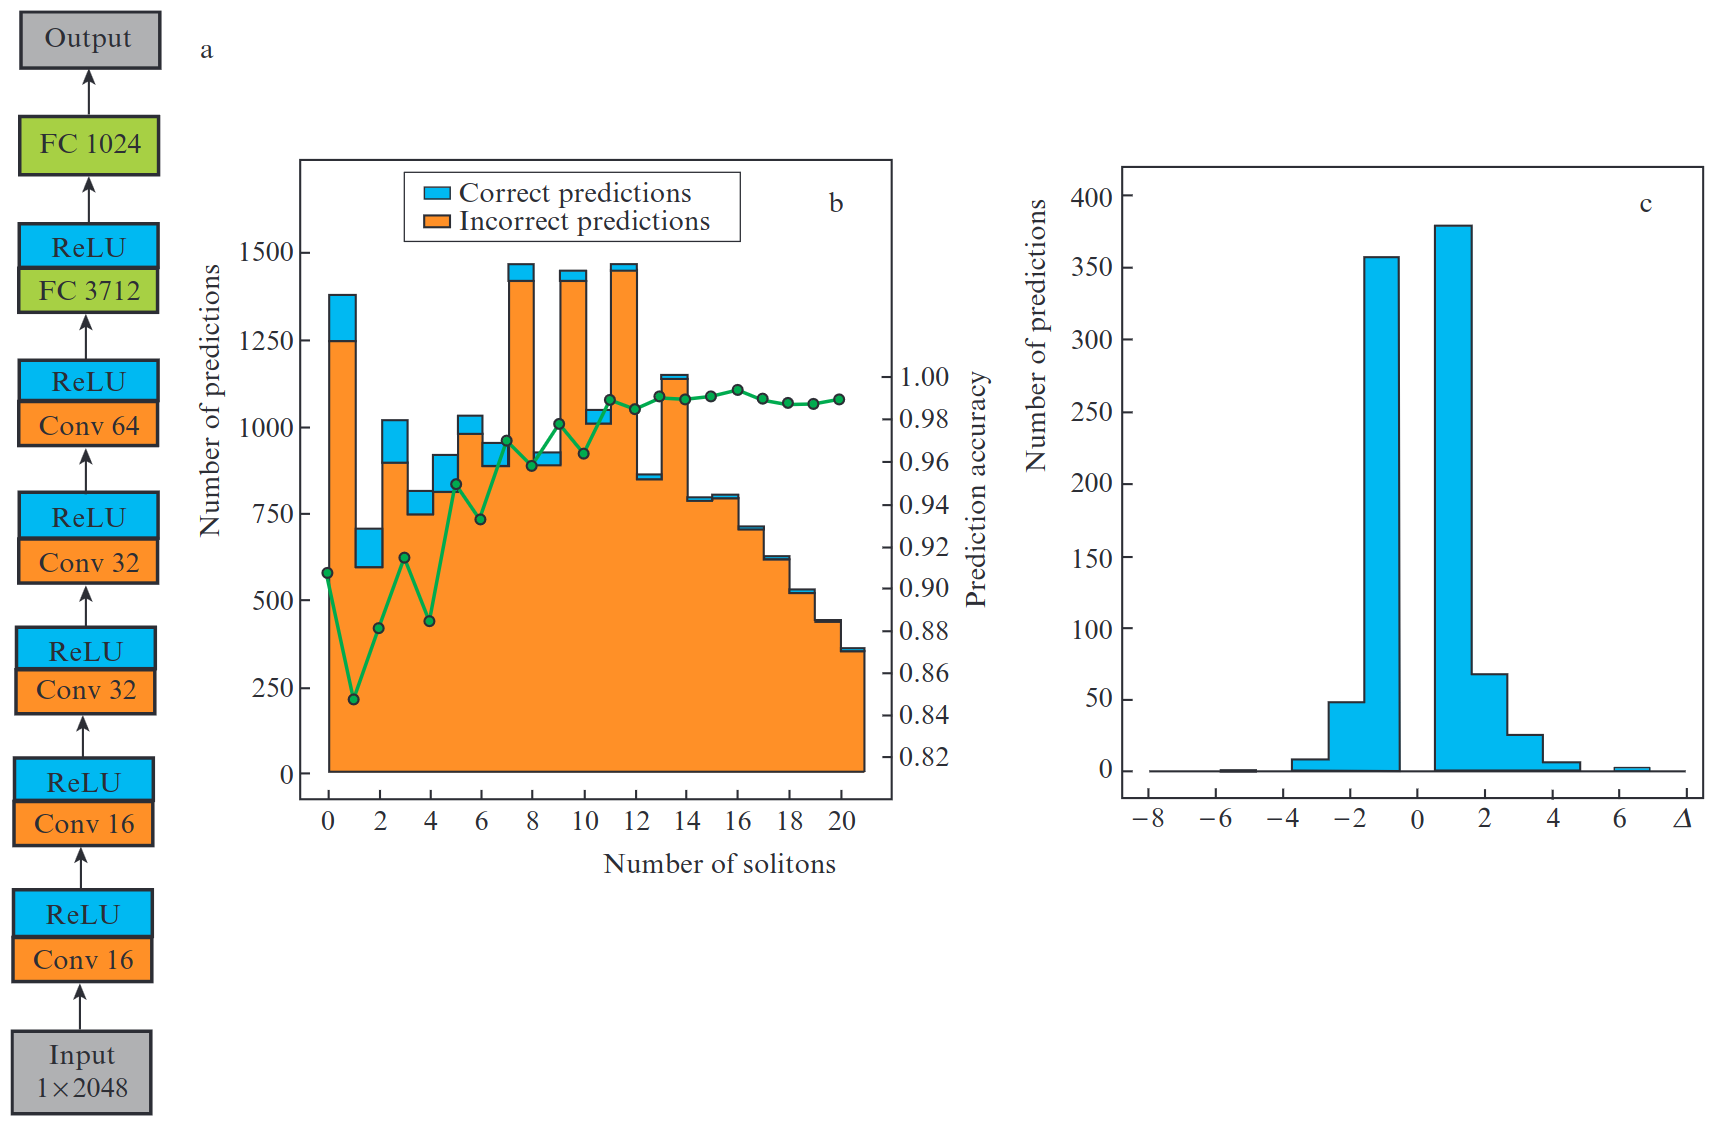
\includegraphics[width=1.0\linewidth]{images/nn_discrete/discrete_result.png}
    \caption{\textbf{(a)} Neural network architecture for predicting the number of discrete eigenvalues (solitons) in the \acrlong{nf} spectrum for a \acrshort{wdm} signal. \textbf{(b)} the distribution of correct and incorrect predictions of the neural network as a function of the number of solitons in signals from the validation sample (the green curve shows the network prediction accuracy for each set of signals with the same number of solitons), and \textbf{(c)} the distribution of the deviation $\Delta$ of the predicted number of solitons in the signals from the validation sample versus their actual
number.}
    \label{fig:nn_discrete_result}
\end{figure}

In total, the training set consists of 174 847 generated signals, which contain from 0 to 20 solitons. The exact number
of solitons in each signal was preliminarily calculated using
a modification of the method of contour integrals,
where the grid step in the spectral space was adaptively calculated depending on the number of solitons in the signal.
To speed up the learning process on the training data set, for
each signal we calculate only the number of discrete eigenvalues in the nonlinear spectrum, rather than the numerical
value of each of the discrete spectral parameters corresponding to the soliton mode. A set of data with complete information on the nonlinear spectrum for each signal will be
considered in subsequent works. The accuracy of network
predictions was determined using a validation set of
19 427 signals (10 \% of the total training set). The network
was trained for 300 epochs, and the final prediction accuracy
on the validation set was 95.39\%. In the training process, we
use for optimisation the Adam algorithm (adaptive moment
estimation). The learning rate was varied during the training
process from $10^{-3}$ at the beginning to $10^{-5}$ at the end. 
Its further reduction did not lead to an increase in the prediction
accuracy.
Figure~\ref{fig:nn_discrete_result}b shows the distribution of correct and incorrect
neural network predictions as a function of the number of
solitons in the signal for the validation sample. The green
curve shows the neural network accuracy as a function of the
number of solitons. The network worked best for signals
where the number of solitons was greater than 10. For such
cases, the accuracy exceeded 98\%. Signals with a single soliton component were processed the worst, with an accuracy of
84\%. In this case, the maximum ‘error’ of the network operation (the difference between the real number of solitons in the
signal and the soliton number predicted by our neural network) was 8 (Fig.~\ref{fig:nn_discrete_result}c). Negative error values correspond to the
case when the network predicts a smaller number of solitons
in the signal than the true number, and positive values occur
when the neural network predicts a larger number of solitons
than is present in the signal. Figure~\ref{fig:nn_discrete_result}b shows the distribution
of the deviation of the predicted number of solitons in the
signals generated by the validation sample from their actual
number: most of the incorrect results are in the range [–2; 2].
Thus, the neural network’s prediction often deviates by a
small value. This means that it captures general features indicating the number of solitons but cannot fully identify particular features. Obviously, with an increase in the number of
convolutional layers, the neural network will be able to determine the internal features of signals more accurately, which
means that its accuracy can be improved. The results show
that neural networks have a great potential for implementing
various stages of \acrshort{nft} with their help.

% \subsection{Conclusion}
% Thus, machine learning and neural network are modern technologies that are actively explored in nonlinear signal processing and for optical communication. The proposed neural network architecture demonstrates the fundamental possibility of its application for the analysis of complex optical signals. This opens up prospects for improving existing systems
% without the need for a deep understanding of the internal
% nonlinear processes that affect the signal transmission quality. We have found that modern neural networks can determine the internal structure of optical signals, and therefore
% can be used as a practical tool for their analysis. This stage is
% undoubtedly only the beginning of research on the possibility
% of using neural networks for optical communication. A promising direction is the development of autoencoders that will
% not only generate optical signals with the necessary parameters, but also select the optimal modulation and encoding formats. We stress that the method proposed in this work is only
% the first step in the development of machine learning methods
% for studying optical signals. The obtained results demonstrate
% that even a network with a small number of trainable parameters can identify complex nonlinear structures of optical signals with high accuracy.